% TODO fill in your paper title
\newcommand{\PaperTitle}{Web Traffic Classification with Extremely Randomized Trees}
\newcommand{\PaperSubtitle}{CSCI434 COLL 400 Capstone Project}
% TODO fill in your paper number when you get it
\newcommand{\PaperNumber}{XXX}

\documentclass[10pt,sigconf,letterpaper,nonacm]{acmart}

%%%%%%%%%%%%%%%%%%%%%%%%%%%%%%%%%%%%%%%%%%%%%%%%%%%%%%%%%%%%%%%%%%%%%%%%%%%%
% This is the preamble; include packages as you see fit.
% Here are a few recommendations:
% \usepackage{color}
% \usepackage{graphicx}
% \usepackage[labelformat=simple]{subcaption}
% \usepackage{xspace}
% \usepackage{multirow}
% \usepackage{tabularray}
% \usepackage[ruled,vlined]{algorithm2e}
% \usepackage{ulem}
% \normalem

%%%%%%%%%%%%%%%%%%%%%%%%%%%%%%%%%%%%%%%%%%%%%%%%%%%%%%%%%%%%%%%%%%%%%%%%%%%%

\begin{document}

\title{\PaperTitle}
\subtitle{\PaperSubtitle}

\author{Ramsey Jooss}
\email{rrjooss@wm.edu}
\affiliation{
  \institution{William \& Mary}
  \city{Williamsburg}
  \state{Virginia}
  \country{USA}
}

\begin{abstract}
  A clear and well-documented \LaTeX\ document is presented as an
  article formatted for publication by ACM in a conference proceedings
  or journal publication. Based on the ``acmart'' document class, this
  article presents and explains many of the common variations, as well
  as many of the formatting elements an author may use in the
  preparation of the documentation of their work. A cite so this compiles~\cite{geneva}.
\end{abstract}

\keywords{Decision and regression trees, Ensemble methods, Extremely randomized trees,
Machine Learning, Network Traffic Classification}

\maketitle

\section{Introduction}
Traffic classification "is instrumental to a number of activities that are of extreme
interest to carriers, Internet service providers and network administrators
in general"~\cite{Valenti2013}. Networking's ubiquity, and the role it play's therein
means traffic classification is a vital consideration across contexts and domains.
"Indeed, [it] is the basic block that is required to enable any traffic management
operations, from differentiating traffic pricing and treatment (e.g., policing, shaping,
etc.), to security operations (e.g., firewalling, filtering, anomaly detection,
etc.)"~\cite{Valenti2013}. The variation across contexts means possible approaches to the
problem also vary, both across time and domain.
\par In cloud computing (specifically in  the context of micro-service architecture)
envisiaging service meshes as a new layer in the network stack has been proposed. "Lower
layers[visibility is limited] due to lacking contextof API calls, encryption, and"
multiplexing or API aggregation among other things. Limited visibility means less knowledge
of applications' needs and therefore less responsiveness to them in this network-intensive
context~\cite{Ashok2021}.
\par At the same time old methods like port-based classification and payload-based
classification are becoming less
possible with the proliferation of encyption and use of non-standard or random
ports~\cite{Valenti2013}. The former applies to web traffic, while an analagous issue
exists for the latter in the prevalence and diversity of web traffic. In response and particularly
empowered by the diverse nature of
web services, and correspondingly their traffic, statistical classification, done on the packet or
behavioral level, can be leveraged~\cite{Valenti2013}.
\par This project collected a dataset of packet capture records of web traffic from:
Google.com, Github.com, Yahoo.com and GeeksforGeeks.com. First this data was split into
training and test sets in a 8:2 ratio. An extremely randomized forest
model was used for classification~\cite{Geurts2006} with two resampling methods for
validation: Bootstrap sampling and repeated k-Fold Cross Validation~\cite{Nakatsu2021}.
\par The goal of this project is to apply machine learning techniques and tools from
elsewhere alongside knowledge learned in CSCI434 to a real-world scenario.

\section{Method}
\begin{figure*}
  \caption{Data Preparation Pipeline}
  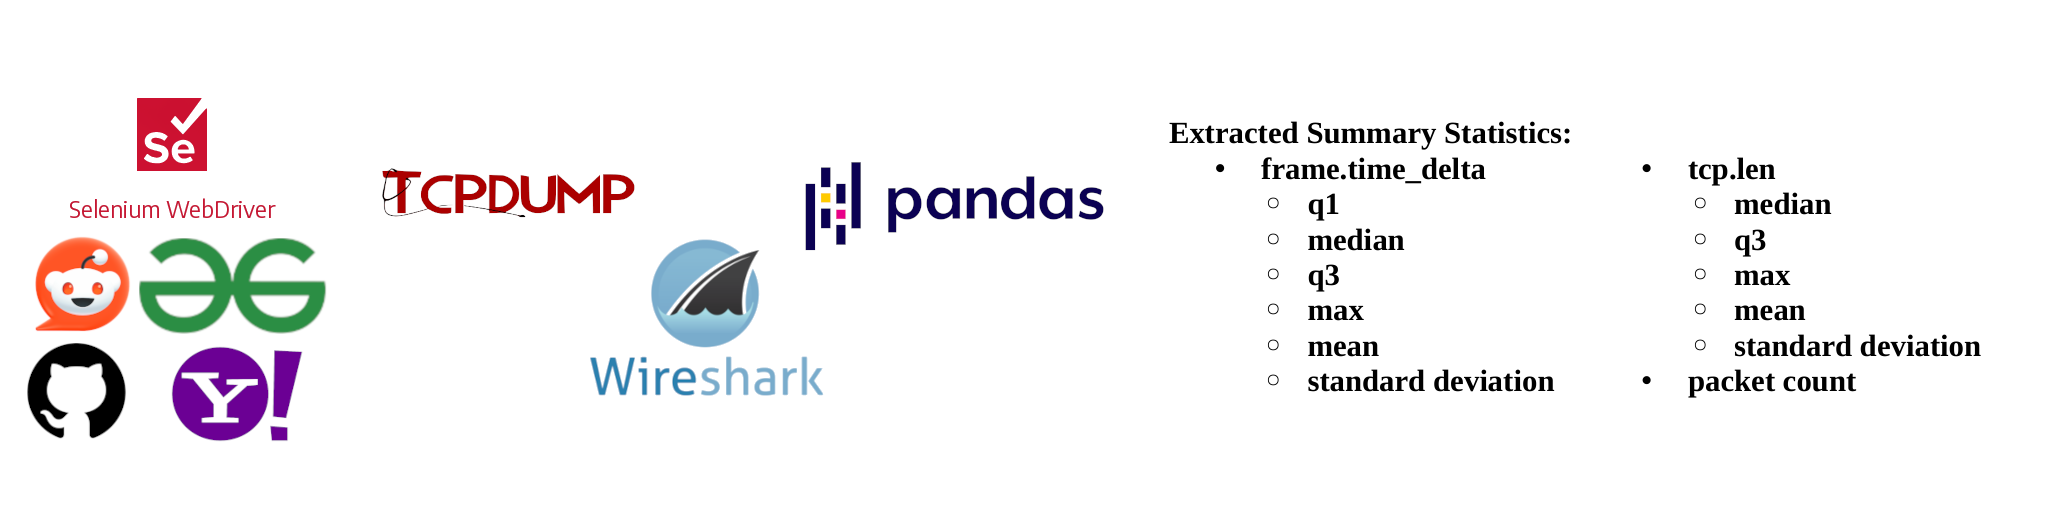
\includegraphics[width=\textwidth]{./DataPreparation.png}
\end{figure*}

\subsection{Data Preparation}
This section presents the methodology for generating, analyzing and classifying web
traffic based on its originating domain. This pipeline is depicted in Fig 1.

\subsubsection{Target Enumeration} To generate a diverse targets for each of the target
domains two methods were used sitemap parsing and spiderfoot~\cite{Spiderfoot}. The
python package \textit{Ultimate Sitemap Parser}~\cite{USP2025} was used for generating
lists of pages from Google.com, Yahoo.com and GeeksforGeeks.com. However, this method was
not possible for Github.com since it lacks a sitemap. Instead, the open source
intelligence (OSINT) automation tool Spiderfoot was used.
\par These techniques generated many thousands of locations for each domain. Using all of
these would be unfeasible for the scope of this project to they were arbitrarily reduced
to a random subset for each domain, totaling 495 urls.

\subsubsection{Traffic Generation} Web traffic generation for
systematic analysis poses an issue as manual web browsing is difficult at scale and risks
the consistency of data,
conversely naive programatic approaches of generating http(s) request fail to emulate
real web browsing. To programatically generate realistic web traffic this project uses
Selenium WebDriver, "commonly referred to as just \textit{WebDriver}"~\cite{Selenium2024}.
\par"WebDriver drives a browser natively, as a user would, either locally or on a remote
machine using the Selenium server" ~\cite{Selenium2024}. This project uses WebDriver
locally because of it's limited scope, but leveraging the Selenium server may be useful
for more extensive data collection. For the sake of simplicity this project opted for the
simple emulation of loading the enumerated locations so only a subset of WebDriver's
features were used. Still, it's feature set provided an important tools for the task. One
of "the most common challenge for browser automation is ensuring that the web application
is in a state" before executing a particular command to avoid race
conditions~\cite{Selenium2024}. To address this WebDriver provides a diversity of waiting
strategies~\cite{Selenium2024}, which this project uses to ensure the normal course of
page loading is captured. The start and end epoch times for each target's web traffic was
recorded so captured traffic's could be associated with it's source.
\subsubsection{Traffic Capture} To capture the generated network traffic
\textit{tcpdump}~\cite{Tcpdump} was used. Tcpdump is based on
libpcap~\cite{Tcpdump}, the same library wireshark uses to capture live network
data~\cite{WiresharkLibpcap}. The choice between these utilities is arbitrary.

\subsubsection{Feature Engineering} Wireshark's cli TShark~\cite{Wireshark} was used to
filter and extract timing and size details about each captured packet. Specifically the
fields frame.time\_epoch, frame.time\_delta, and tcp.len were captured.
\par The pandas package~\cite{pandas} was used to first associate each packet data entry
with it's originating target and then to generate summary staistics of each target's set
of entries. In addition to counting the number of packets for each target quartile range
data, as well as mean and standard deviation for time deltas and tcp packet length were
calculated. Summary statistics that were constant across all recorded entries were
removed as they cannot be useful for categorization. Mode was not included for this reason since
\par This step was lossy resulting in a limited data set of traffic from 258 targets, this
could be the result of errors at either the Traffic Capture, or Feature Engineering
stages but both were costly in terms of time so deeper analysis is not available at this
time. The distribution of these records can be seen in Table 1.

\begin{table}
  \caption{Resulting Records}
  \begin{tabular}{cc}
    Domain & Count \\
    \midrule
    Google.com & 68\\
    Github.com & 71\\
    Yahoo.com & 57\\
    GeeksforGeeks.com & 62
  \end{tabular}
\end{table}

\subsection{Machine Learning for Classification}
\subsubsection{The Extra-Trees Algorithm} "Ensemble methods combine the
predictions of several base estimators built with a given learning algorithm in order to
improve generalizability / robustness over a single estimator"~\cite{sklearn111}. A
traditional example of this is the random forests algorithm. "During the construction of
each tree in the forest, a random subset of the features is considered"~\cite{sklearn111}
and the most discriminative threshold is chosen for that node. The constructed trees are
individually overfit which can lead to high variance, sensitivity to fluctuations in
training data~\cite{sklearn111}. The final prediction is derivate by aggregating the
outputs of an ensemble of unpruned trees via majority vote for classification or via
averaging for regression~\cite{Geurts2006}
\par Extra-Trees (Extremely Randomized Trees) is another ensemble learning method for
regression or classification that extends the concept of randomized decision trees.
Unlike traditional tree-based ensemble methods like Random Forests, Extra-Trees
introduces a higher degree of randomization by selecting both the attribute and cutoff
point entirely at random rather than optimizing split points locally towards maximizing a
criterion~\cite{Geurts2006} "This usually allows to reduce the variance of the model a
bit more, at the expense of a slightly greater increase in bias"~\cite{sklearn111}. The
scikit-learn python package's ExtraTreesClassifier class~\cite{sklearn111} was used to apply
this algorithm.

\subsubsection{Validation Methods} The two resampling methods used in this project are
k-fold cross validation and bootsrap resampling. Emperical investigation suggests k-fold
cross-validation exhibits lower variance than the bootstrap method~\cite{Ljumovic2015}.
Unfortunately this projects implementation does not lend itself to direct comparison
because of the structural difference of implementation in the scikit-learn python package.
\par\textbf{The Bootstrap Method.} Bootstrap resampling "randomly generates training and
validation sets" by randomly selecting rows of the training set with
replacement~\cite{Nakatsu2021}. This means that entries can be repeated in the final
training set and the validation set consists of entries in the training set not contained
in the final training set.
\par This validation method was employed by passing an argument to the
ExtraTreesClassifier constructor.
\par\textbf{k-Fold Cross Validation.} "K-fold cross-validation assumes randomly
dividing a dataset into k folds or parts of roughly equal size. The k-th fold is used as
a validation set and the remaining k-1 folds are used for training the model. This
procedure is repeated k times, and each time a different fold is used as validation
set"~\cite{Ljumovic2015}. "After iterating k times this way, an average of the k
validation errors is calculated so that, again, a more accurate estimate of error rate
can be obtained"~\cite{Nakatsu2021}. This accuracy allows for comparing the results of varied
parameters for the Extra-Trees algorithm to increase model accuracy.
\par This method was employed by using scikit-learn's GridSearchCV
algorithm~\cite{sklearn111}. The parameter grid used, and the default values for those
parameters are shown in Table 2.

\begin{table}
  \caption{Arguments}
  \begin{tabular}{c|c|c}
    ExtraTreesClassifier & Default & Parameter Grid\\
    Parameter & Value & Options\\
    \midrule
    n\_estimators & 100 & 10, 20, 50, 100, 200\\
    max\_depth & None & None, 5, 10, 20, 30\\
    min\_samples\_leaf & 1 & 1, 5, 10\\
    min\_samples\_split & 2 & 2, 5, 10\\
    bootstrap & False & True, False
  \end{tabular}
\end{table}

\section{Evaluation}
\begin{table*}
  \caption{Summary of Results of 50 Runs}
  \begin{tabular}{c|c|c|c}
    Method & Avg Acc. & Acc. $\sigma^2$ & Most Common Final Parameters \\
    \midrule
    k-Fold & 78.0\% & 0.00378 & bootstrap: False, max\_depth: None, min\_samples\_leaf: 2,
    min\_samples\_split: 5, n\_estimators: 50\\
    Bootstrap & 77.5\% & 0.00229
  \end{tabular}
\end{table*}

\par The summary of 50 runs with each validation method are shown in Table 3. Accuracy
was tracked because it was used as the scoring parameter for GridSearchCV. These results
suggest that this implementation's k-Fold validation is insigificantly more accurate than
the bootstrap method alone, but bootstrap resampling exhibited lower variance in accuracy.
\par Since the split between training and testing data is a randomized 3:1 split for each
run, and both the bootstrap method and k-fold cross-validation heavily depend on the
representativeness of training data, averaged data is more likely to give an accurate
picture of the effectiveness of each approach than range data given the limited data
set~\cite{Ljumovic2015}. The similarity of the results between the two methods could
suggest a limitation of the testing data. While the diversity of web traffic makes
statistical methods of
categorization all the more imperitive, categorization at the domain level still leaves a
large diversity of traffic in each category.

\section{Conclusion \& Future Work}
\par Structurally, further developing the implementations for both the bootstrap and
k-fold methods for better comparability is needed. Additionally other techniques for
summarizing network behavior are needed. This could include cluster analysis, regression
to match more complex patterns, and particularly in the interest of real world
applicapility statistics dependent on order and overall timing. Developing this more
complex analysis would pair well with more complex interactivity in generating web
traffic or finding real-world sources of data as techniques would likely have to be tuned
to, and selected for, particular data patterns.
\par Further analysis of data collection methods is needed to improve it so a more
diverse dataset can be efficiently compiled as to support even further analysis. Varying
scales and diversity of data is only one axis along which further comparion of validation
methods is needed. More measures of model fit also need to be considered such as
precision, recall, and measures considering resultant forest / tree structures and
prediction confidence.
\par The code for this project can be found at
\href{https://github.com/rrjooss/CSCI434-CapstoneProject}.

% Note from the CFP that this section must include a statement about
% ethical issues; papers that do not include such a statement may be
% rejected.

%%%%%%%%%%%%%%%%%%%%%%%%%%%%%%%%%%%%%%%%%%%%%%%%%%%%%%%%%%%%%%%%%%%%%%%%%%%%
% We're in the endgame now

\bibliographystyle{ACM-Reference-Format}
\bibliography{refs}

\end{document}
